%%%%%%%%%%%%%%%%%%%%%%%%%%%%%%%%%%%%%%%%%%%%%%%%%%%%%%%%%%%%%%%%%%%
% Method
% Team:
% Union
% Members: 
% Bernie Huang, Jim Lan, Hoang Tan, Kenny Hsu, Rahul Aditya, Tan Phat, Wei
% Relative files:
% Method_Union.tex
% Note:    
% Do not compile this file compile Main.tex to get the pdf file instead.
%%%%%%%%%%%%%%%%%%%%%%%%%%%%%%%%%%%%%%%%%%%%%%%%%%%%%%%%%%%%%%%%%%%
\section*{Method}
As mentioned in the background, our group use natural language processing in order to generate metadata. 
The scope of metatada processing is about producing at least three types of metadata include author name, title and abstract. 
This is the least we want to produce within the time frame of this course. 
Once accomplishing the 3 types of metadata, we will extend the scope of our project, intimidate the scheme to produce other remaining metadata such as doix number, journal name, volume number and so on. 
If time is still on our side, we will even extend the scope our project further and join other teams to produce a search engine. 
Following discussion are our plan to complete extracting the 3 first types of metatata from PDF files.
\subsection*{Title extraction}
We chose python to be the program to catch the title and other metadata as well. First step, we import some necessary packages and functions as following:
\begin{enumerate}
	\item re: Regular expression package
	\item os: This function can connect the python to operating system, so that we can call the path
	\item nltk: A natural language toolkit. We use the corpus plaintext function to build the txt file in a folder as corpus.
	\item string:The string package includes a lot of classes such as lowercase, uppercase,punctuation,digits or whitespace...etc. 
\end{enumerate}  
To begin, we convert all PDF files we want to deal with into a txt file and set the path and store them in specific folder. 
Then, regular expression in python can help capturing the first sentence in the txt files, which have been converted and stored in specific folder in previous step. 
Afterward, we intend to produce the title of the article in a txt file.   

\subsubsection*{Author extraction}


\subsubsection*{Abstract extraction}
	Developing from previous theory mentioned in the background section, we use the python to catch the abstract. The following step is below
	%\begin{center}
	%	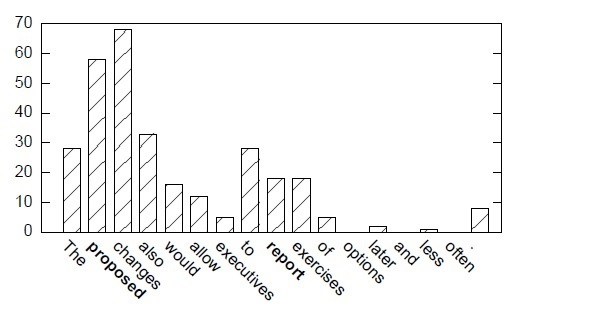
\includegraphics[width=\columnwidth]{Union_Background_Chart_2}
	%\end{center}
	The pdf is converted into txt file.Thus, it will create the txt file. The work is done by hand coding. For detailed coding scheme, we have presented it in the appendix at the end of this report\\ 
	After being able to read the txt file on every line, the python will detect the content of the abstract. In order to do so, we strip the text between "abstract" label and "introduction" label.\\ 	
	abstract-database:including the condition\\
	1. capital         "ABSTRACT"\\
	2. lower case      "abstract"\\
	3. in the sentence "Abstract—Word sense ....."\\
	4. and so on \\
	In the process building "abstract database", we are aware of different papers may have different form of structures and writing style, we search through numbers of articles from different journals. Number of article found is 100, from 20 different journals including The Lancet, Progress in Energy and Combustion Science, Chemical Analysis and so. Search results for sections such as Theoretical, Methods, Results, Discussion, Conclusion, Acknowledgements are also obtained.  Table below are the results of the search.\\
	\begin{center}
		%\includegraphics[width=\columnwidth]{Table for method Union}.\\
		%\includegraphics[width=\columnwidth]{Table 2 for method Union}.\\
		%\caption{Result of finding all forms of "abstract", "introduction" written by different authors}
	\end{center}
	Then our program will read the txt file on every line.If the python detects the abstract-database-stop's words ,it will stop to catch the sentences.\\ 
	abstract-database-stop:including the following conditions
	1. the blank line
	2. specific words in the beginning "Keywords"
	3. and so on.\\
	The intended output are sentences extracted to the txt file. To further validate if the program can run precisely, members randomly search for articles (10 articles) to test the programs. The program was run successfully and all abstracts was extracted from the text. \\ 	
	

\subsubsection*{Search sentences}
\begin{itemize}
	\item I use python to complete the task. 
	\begin{center}
		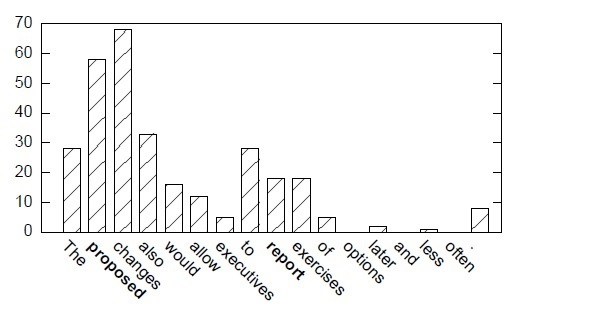
\includegraphics[width=0.8\columnwidth]{Union_Background_Chart_2}
	\end{center}
	\item First,turn the PDF to the txt file .(Make the programe easy to read file)\\ 
	\item Second,read the txt file by lines.\\ 	
	\item Third,create the array to divide the section of the articles.\\ 	
	\item Forth,expend the array to divide the section clearly.\\ 	
	\item Fifth,Users search the sentence.The programe search all sections by this sentence.\\
	\item Sixth,Show the results\\  		
	
\end{itemize}
Our project has four remaining weeks to complete (counting from 26 May 2016). 

\newpage % Ends the current page and causes all figures and tables to be printed